\documentclass{beamer}
\usepackage[utf8]{inputenc}
\usepackage[T1]{fontenc}
\usepackage[francais]{babel}

\usepackage{graphicx}
\usetheme{Frankfurt}
\usecolortheme{dove}

\usepackage{xcolor}
\definecolor{red}{rgb}{0.5,0,0}
\definecolor{green}{rgb}{0,0.5,0}

\title{Presentation de rssint}
\author{Anas Alaoui \and Romain Bressan}
%\date{31 août 2015}

\addtobeamertemplate{navigation symbols}{}{ \hspace{1em}    \usebeamerfont{footline}%
    \insertframenumber / \inserttotalframenumber } %page number inside nav bar

\begin{document}
\frame{\maketitle}
\section{Contexte}
\frame{
	\frametitle{Objectifs}
	Réaliser un système de veille sur Internet qui exploite des flux RSS.
	\begin{itemize}
		\item Lecteur de flux RSS et ATOM
		\item Collecteur : conversion (extraction de texte), encodage,
			langue, stemmer, boilerplate
		\item Indexeur : Lucene
		\item Requeteur : recherche dans l'index
		\item Classifieur : classer un document à partir des documents
			déjà classés avec KNN
	\end{itemize}
}
\frame{
	\frametitle{Flux RSS}
	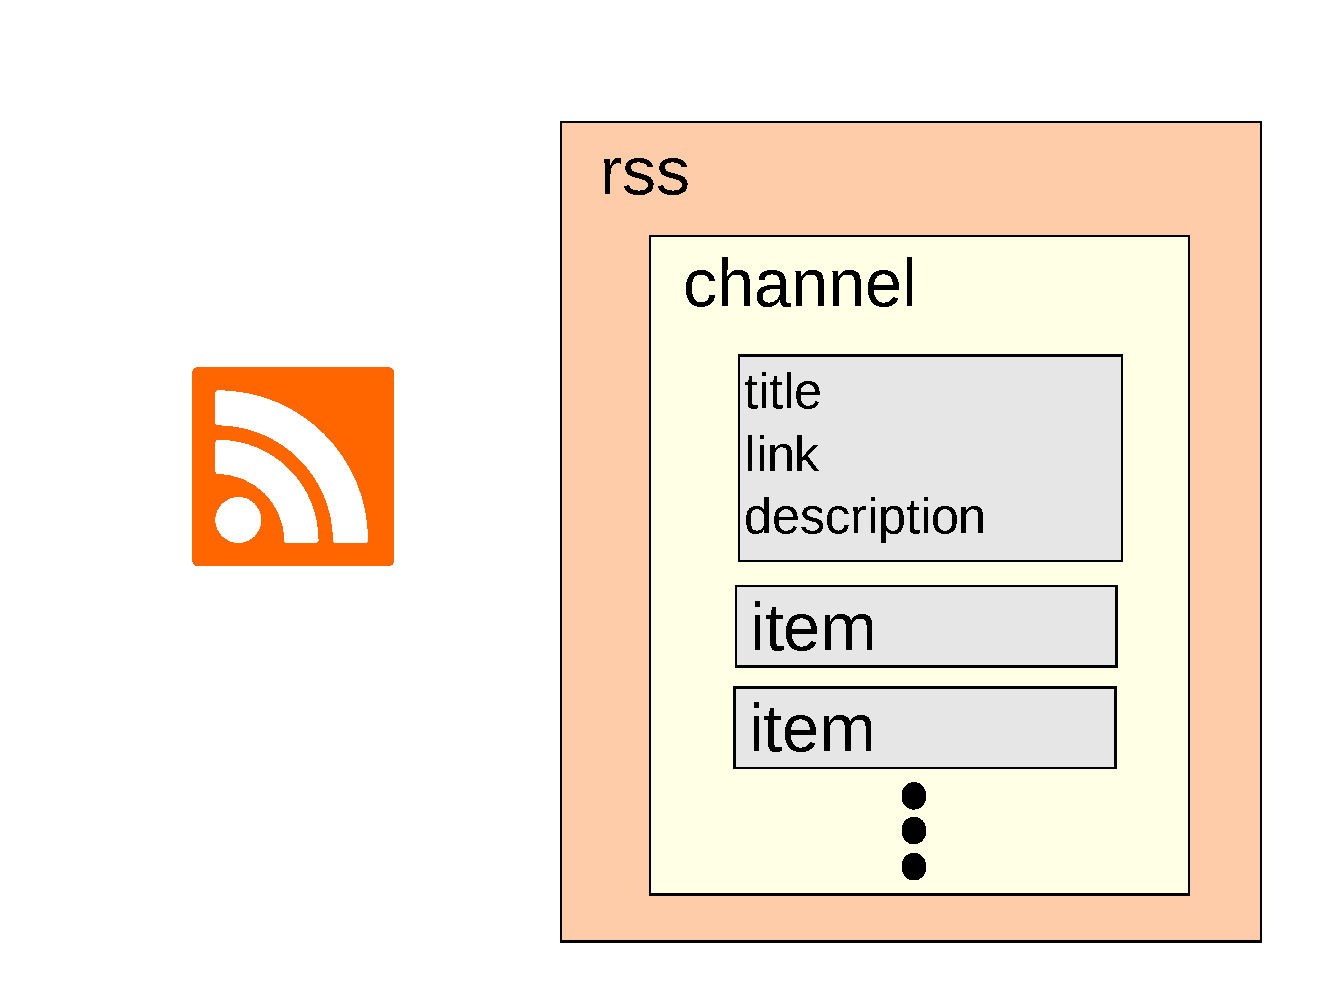
\includegraphics[width=\textwidth]{rss.pdf}
}
\section{Solution}
\frame{
	\frametitle{Architecture}
	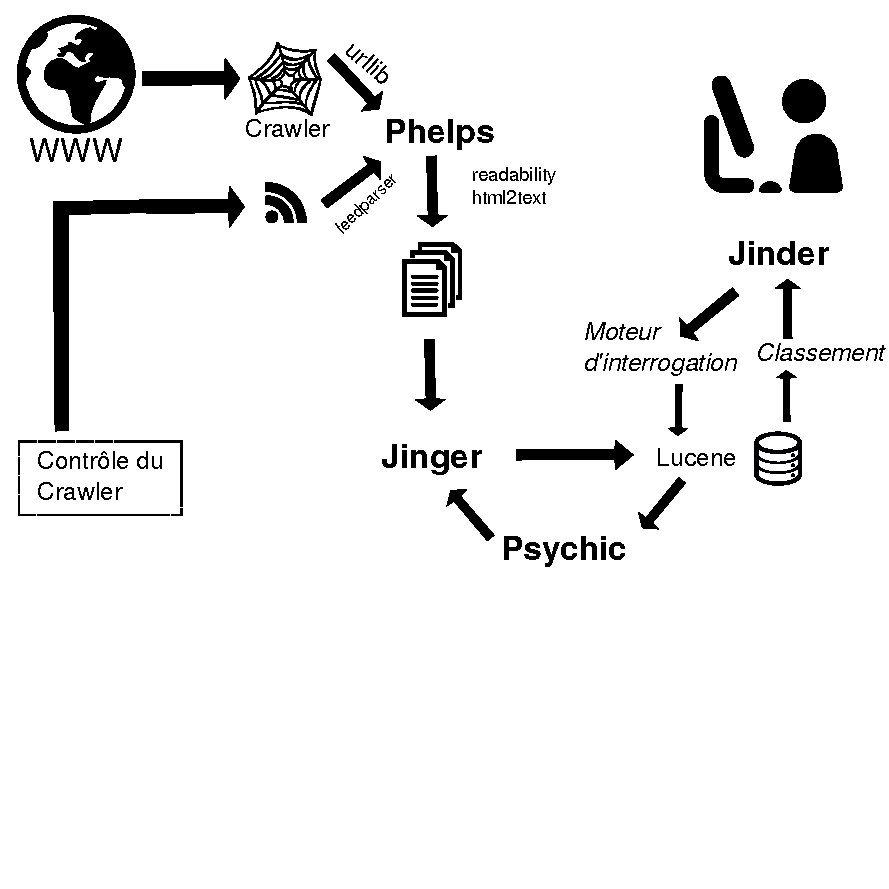
\includegraphics[width=\textwidth]{archi.pdf}
}
\frame{
	\frametitle{Dépendances}
	\begin{itemize}
		\item feedparser, Python, BSD 2-Clause
		\item html2text, Python, GNU GPL 3.0
		\item readability, Python, Apache License 2.0
		\item lucene, Java, Apache License 2.0
	\end{itemize}
}
\frame{
	\frametitle{Travail rendu}
	\begin{itemize}
		\item Lecteur de flux \textcolor{green}{RSS} et \textcolor{green}{ATOM}
		\item \textcolor{green}{Collecteur} :
			\textcolor{green}{conversion (extraction de texte)},
		        \textcolor{green}{encodage},
			\textcolor{red}{langue}, \textcolor{red}{stemmer},
			\textcolor{green}{boilerplate}
		\item \textcolor{green}{Indexeur} : Lucene
		\item \textcolor{green}{Requeteur}: recherche dans l'index
		\item \textcolor{green}{Classifieur} : classer un document
			à partir des documents déjà classés avec KNN
	\end{itemize}
}
\section{Démonstration}
\frame{
	\frametitle{Démonstration}
}
\end{document}
